\documentclass[9pt,twoside,lineno]{pnas-new}
% Use the lineno option to display guide line numbers if required.

\usepackage{xr-hyper}
\externaldocument{manuscript_noSI}

\templatetype{pnassupportinginfo}
% \readytosubmit %% Uncomment this line before submitting, so that the instruction page is removed.

\title{Deep mutational scanning of hemagglutinin helps predict evolutionary fates of human H3N2 influenza variants}
\author{JM Lee, J Huddleston, MB Doud, KA Hooper, NC Wu, T Bedford, JD Bloom}
\correspondingauthor{Trevor Bedford \\ tbedford@fredhutch.org \\ Jesse D. Bloom \\ jbloom@fredhutch.org}

\begin{document}

%% Comment/remove this line before generating final copy for submission
%\instructionspage  

\maketitle

%% Adds the main heading for the SI text. Comment out this line if you do not have any supporting information text.
\SItext

\subsection*{Codon mutagenesis}
The codon-mutant libraries were generated in the Perth/2009 HA-G78D-T212I background using the PCR-based approach described in \cite{bloom2014experimentally} with the primer melting-temperature modifications described in \cite{dingens2017comprehensive}, using two rounds of mutagenesis.
The script to design the mutagenesis primers is at \url{https://github.com/jbloomlab/CodonTilingPrimers}.
We created three independent libraries, one for each biological replicate.
The mutant variants were then cloned at high efficiency into the pICR2~\cite{ashenberg2017deep} vector using digestion with BsmBI, ligation with T4 DNA ligase, and electroporation into ElectroMAX DH10B competent cells (Invitrogen 18290015).
We obtained $>$6 million transformants for each replicate.
We scraped the plates, expanded the cultures in liquid LB (Luria-Bertani Broth) + ampicillin at 37$^{\circ}$C for 3 h with shaking, and then maxiprepped.
We randomly chose 31 clones to Sanger sequence to evaluate the mutation rate (see SI Appendix, Figure~S2).

\subsection*{Barcoded-subamplicon sequencing}
We generated the HA PCR amplicons for the three plasmid libraries, the three virus libraries, the wildtype plasmid control, and the wildtype virus control using KOD Hot Start Master Mix (EMD Millipore 71842) using the PCR reaction mixture and cycling conditions described in~\cite{bloom2014experimentally} and the P09-HA-For and P09-HA-Rev primers.
We prepared the sequencing libraries using a barcoded-subamplicon strategy~\cite{wu2014high} to increase the accuracy from deep sequencing.
The exact details of this approach are described in~\cite{doud2016accurate} (also see \url{https://jbloomlab.github.io/dms_tools2/bcsubamp.html}).
The primers used to generate the subamplicons are in the SI Appendix (Dataset~S2).
We performed deep sequencing on a lane of an Illumina HiSeq 2500 using 2 $\times$ 250 bp paired-end reads in rapid-run mode.

\subsection*{Phylogenetic model comparison and fitting of a stringency parameter}
For the analysis in Table~\ref{tab:phydms}, we downloaded all full-length H3 HA sequences from the Influenza Virus Resource~\cite{bao2008}, and randomly subsampled two sequences per year.
These sequences were aligned using MAFFT~\cite{katoh2013mafft} and used to infer a phylogenetic tree using RAxML~\cite{stamatakis2006raxml} with a GTRCAT model of nucleotide substitution.
We then used \texttt{phydms}~\cite{hilton2017phydms} (\url{https://github.com/jbloomlab/phydms}, version \texttt{2.2.2}) to fit the substitution models listed in Table~\ref{tab:phydms}.

The amino-acid preferences were re-scaled by the stringency parameter using the approach described in \cite{hilton2017phydms}.
Note that the re-scaling simply puts the amino-acid preferences on a useful scale for visualization in logo plots, and has no effect on any of the quantitative conclusions relating the deep mutational scanning to natural evolution.
The reason is that all of these conclusions use the effects of mutations as calculated using Equation~\ref{eq:muteffect}, and the re-scaling simply acts as a constant multiplier on all mutational effects (e.g., a scale factor) when re-scaled preferences are converted to mutational effects.

The phylogenetic tree of HA subtypes in Figure~\ref{fig:distance_distribution}A was generated as described in~\cite{doud2018quantifying}.

\subsection*{Inference of human H3N2 phylogenetic tree and calculation of maximum mutation frequencies}
To generate the tree shown in the SI Appendix (Figure~S8), we applied Nextstrain's augur pipeline~\cite{Hadfield224048} (\url{https://github.com/nextstrain/augur}; commit \texttt{006896d}) to publicly available H3N2 HA sequences from GISAID \cite{shu2017gisaid} (see the SI Appendix, Dataset~S4), sampling six viruses per month over the time interval of January 1, 1968 to February 1, 2018.
We aligned the resulting 2,189 HA sequences with MAFFT v7.310~\cite{katoh2013mafft} and constructed a maximum likelihood phylogeny from this alignment with RAxML 8.2.10~\cite{stamatakis2006raxml}.
Ancestral state reconstruction and branch length timing were performed with TreeTime~\cite{Sagulenko2018}.
The phylogenetic tree is available as a JSON file on GitHub at \url{https://github.com/jbloomlab/Perth2009-DMS-Manuscript/blob/master/analysis_code/data/flu_h3n2_ha_1968_2018_6v_tree.json.gz}.
The tree was visualized using BALTIC (\url{https://github.com/blab/baltic}).

% notation for frequencies model
\newcommand{\dx}{\mathrm{d}x}						% change in x
\newcommand{\dy}{\mathrm{d}y}						% change in y
\newcommand{\dt}{\mathrm{d}t}						% change in t
\newcommand{\inertia}{\epsilon}			    % inertia parameter
\newcommand{\normal}{\mathcal{N}}				% normal distribution

The frequency trajectory of each individual mutation on the phylogeny is estimated following Nextstrain's augur pipeline and as first implemented in Nextflu \cite{neher2015nextflu}.
Herein, mutation frequency dynamics are modeled according to a Brownian motion diffusion process discretized to one-month intervals.
The number of viruses sampled in each interval determines the denominator of the mutation frequency calculations.
Relative to a simple Brownian motion, the expectation includes an ``inertia'' term $\inertia$ that adds velocity to the diffusion and the variance includes a term $x(1-x)$ to scale variance according to frequency following a Wright-Fisher population genetic process.
This results in the following diffusion process
\begin{equation}
x(t+\dt) = \normal\big( x(t) + \inertia \, \dx , \; \dt \, \sigma^2 \, x(t) \, (1-x(t)) \big),
\end{equation}
with `volatility' parameter $\sigma^2$.
The term $\dx$ is the increment in the previous timestep, so that $\dx = x(t) - x(t-\dt)$.
We used $\inertia = 0.7$ and $\sigma^2 = 0.05$ to maximize fit to empirical trajectory behavior.

We also include an Bernoulli observation model for mutation presence / absence among sampled viruses at timestep $t$.
This observation model follows
\begin{equation}
f(x,t) = \prod_{v\in V} x(t) \prod_{v\notin V} (1-x(t)),
\end{equation}
where $v\in V$ represents the set of viruses that have the mutation and $v\notin V$ represents the set of viruses that do not have the mutation.
Each frequency trajectory is estimated by simultaneously maximizing the likelihood of the process model and the likelihood of the observation model via adjusting frequency trajectory $\mathbf{x}=(x_1, \ldots, x_n)$.

We also repeated the above analyses using only viruses that were sequenced directly without passaging.
Routine direct sequencing did not begin until the early 2000s \cite{mcwhite2016sequence}.
To construct a tree with a similar number of viruses as the original analysis, we sampled 30 viruses per month between January 1, 2000 and April 1, 2018, producing a tree with 2,374 unpassaged viruses with augur (commit: \texttt{6d9f708}).
We included the passaged DMS strain, A/Perth/16/2009, in the resulting tree to enable comparison between pre-Perth and post-Perth clades.

\subsection*{Analysis of mutational shifts}
To compare the Perth/2009 H3 and WSN/1933 H1 HA preferences, we first aligned the wildtype HA sequences using MAFFT~\cite{katoh2013mafft}.
To quantify the shifts in preference for every alignable site while accounting for experimental noise, we used the approach described in~\cite{haddox2018mapping} and used the RMSD$_{\text{corrected}}$ values as our quantification of the extent of each shift.

For the plots shown in Figure~\ref{fig:RMSD_heatmap}B, any residues falling between Cys-52 and Cys-277 were defined as the head domain, and all other residues were defined as the stalk domain.
We used the multiple sequence alignment of the HA subtype sequences from \cite{doud2018quantifying} to identify sites that are absolutely conserved across all subtypes, or in the different clades described in Figure~\ref{fig:RMSD_heatmap}.

\subsection*{Validation of individual point mutants}
To validate the viral growth of Perth/2009 HA point mutants M(-16)K, C52A, C52C, T24F, T40V, S287A, and C199(HA2)K, we used site-directed mutagenesis to introduce the amino-acid mutation into the Perth/2009 HA bidirectional reverse genetics plasmid, and verified the sequence of two clones for each mutant by Sanger sequencing.
We generated these individual mutant viruses carrying GFP in the PB1 segment using a protocol described in \cite{bloom2010permissive,hooper2013mutant}, and the PB2, PA, NP, NA, M, and NS segments of the A/WSN/1933 (H1N1) strain.
To rescue each mutant GFP-carrying virus in duplicate, we transfected a co-culture of $4 \times 10^5$ 293T-CMV-PB1 and $0.5 \times 10^5$ MDCK-SIAT1-CMV-PB1-TMPRSS2 cells with the eight reverse genetics plasmids and the pHAGE2-EF1aInt-TMPRSS2-IRES-mCherry-W plasmid.
Each well received a transfection mixture of 100 $\mu$L DMEM, 3 $\mu$L BioT transfection reagent, and 250 ng of each plasmid.
We changed the media in each well with 2 mL IGM eight hours post-transfection.
At 53 hours post-transfection, transfection supernatants were harvested, clarified by centrifugation at 2000 $\times$ \textit{g} for five minutes, aliquoted, and frozen at -80$^\circ$C.

To titer the GFP-carrying viruses, we plated $1 \times 10^5$ MDCK-SIAT1-CMV-PB1-TMPRSS2 cells per well in 12-well plates in IGM.
Four hours after plating, we infected cells with dilutions of viral supernatant.
At 16 hours post-infection, we selected wells with 1 to 10\% of cells that were GFP-positive and analyzed the fraction of GFP-positive cells by flow cytometry to calculate the titer of infectious particles per $\mu$L. 


%%% Each figure should be on its own page
\begin{figure}
\centerline{
\includegraphics[width=0.5\textwidth]{figs/supp_G78D-T212I/G78D-T212I.pdf}}
\caption{\label{suppfig:Perth2009_mut}
{\bf Characterization of the G78D-T212I Perth/2009 HA variant.}
(A)
The G78D-T212I Perth/2009 HA variant supports better viral growth than the wildtype Perth/2009 HA.
Viruses were generated in duplicate by reverse genetics with the Perth/2009 NA and WSN internal genes, and passaged once at MOI = 0.01 in MDCK-SIAT1-TMPRSS2 cells.
The rescue and passage viral supernatants were collected at 72 hours post-transfection and 44 hours post-infection, respectively, and titered in MDCK-SIAT1-TMPRSS2 cells.
The points mark each duplicate and the bar marks the mean.
(B)
The D78 variant remained at a low frequency in natural human H3N2 sequences over the past $~\sim$10 years.
The A212 variant rose to fixation in $~\sim$2011, replacing the T212 variant.
}
\end{figure}
\FloatBarrier

\begin{figure}
\centerline{
\includegraphics[width=0.6\textwidth]{figs/supp_SangerSeq/SangerSeq.pdf}}
\caption{\label{suppfig:SangerSeq}
{\bf Sanger sequencing of 31 randomly chosen clones from the mutant plasmid libraries.}
(A) There were an average of $\sim$1.4 codon mutations per clone across the three plasmid mutant libraries.
(B) A mixture of one-, two-, and three-nucleotide mutations were present, with slightly fewer triple-nucleotide changes than expected.
(C) Nucleotide frequencies were uniform in the codon mutations.
(D) The mutations were distributed relatively evenly across the length of the HA coding sequence.
(E) We calculated the pairwise distances between mutations for clones carrying more than one mutation.
The cumulative distribution of these distances is shown in the red line.
The blue line indicates the expected distribution if mutations in multiply mutated genes are randomly dispersed along the sequence.
}
\end{figure}
\FloatBarrier

\begin{figure}
\centerline{\includegraphics[width=0.9\textwidth]{figs/supp_diffprefs/diffprefs.pdf}}
\caption{\label{suppfig:diffprefs_logoplot}
{\bf Sites where there are strong differences between our experimental measurements and the amino-acid frequencies among natural HA sequences.}
We calculated the distance between our H3 measurements and the alignment frequencies using the same approach as in Figure~\ref{fig:distance_distribution}, but using the alignment frequencies in place of the H1 preferences.
For each site, the height of each letter above or below the line indicates how much more or less preferred that amino acid is in our experiments compared to its frequency nature.
The overlays show the same information as in Figure~\ref{fig:logoplot} (domain and wildtype amino acid).
The sites are in H3 numbering.
The HA alignment used to calculate the natural frequencies is the same one used in Table~\ref{tab:phydms}.
}
\end{figure}
\FloatBarrier

\begin{figure}
\centerline{\includegraphics[width=0.4\textwidth]{figs/supp_point_mut_validation/startcodon_titers.pdf}}
\caption{
{\bf Validation that the Perth/2009 HA is somewhat tolerant to mutation of the canonical start codon.}
We created variants of the Perth/2009 HA in which the canonical start codon was mutated (amino-acid mutation M(-16)K, codon mutation ATG$\rightarrow$AAA), a conserved cysteine was mutated to alanine (C52A, codon mutation TGC$\rightarrow$GCA), and the same cysteine was synonymously mutated (C52C, codon mutation TGC$\rightarrow$TGT).
We selected these mutations because our deep mutational scanning results in Figure~\ref{fig:logoplot} surprisingly suggest that the start codon (position -16) is fairly tolerant of mutations, but that site 52 is highly intolerant of mutation to anything other than cysteine.
The synonymous C52C mutation is a negative control mutation that is not expected to have any effect.
We then used reverse genetics to generate viruses carrying the wildtype HA or each point mutant, with GFP packaged in the PB1 segment to enable easy titering by flow cytometry~\cite{bloom2010permissive,hooper2013mutant}.
Each variant was generated in duplicate, and the plots show the viral titer in the supernatant at 53 hours post-transfection.
As expected, the C52A virus is essentially non-viable, while the C52C mutation is roughly equivalent to wildtype.
The M(-16)K mutation is only moderately attenuated, validating that the canonical start codon is not completely essential for viral growth.
}
\label{suppfig:startcodon_validation}
\end{figure}
\FloatBarrier

\begin{figure}
\centerline{\includegraphics[width=0.4\textwidth]{figs/supp_point_mut_validation/glycan_titers.pdf}}
\caption{\label{suppfig:glycan_validation}
{\bf Validation of viral variants with mutations at N-linked glycosylation motifs.}
We created variants of the Perth/2009 HA with mutations that eliminated N-linked glycosylation motifs (Asn-Xaa-Ser/Thr) at asparagine residues 22, 38, and 285 (these are mutations T24F, T40V, and S287A, respectively).
The codon mutations were ACG$\rightarrow$TTC, ACT$\rightarrow$GTA, and AGC$\rightarrow$GCG, respectively.
We then used reverse genetics to generate viruses carrying the wildtype HA or each of these mutants.
Each variant was generated in duplicate, and the plots show the viral titer in the supernatant at 53 hours post-transfection.
The viruses with mutations at the motifs at residues 22 and 38 reached titers at least as high as wildtype, whereas the virus with a mutation to the motif at residue 285 was modestly attenuated.
}
\end{figure}
\FloatBarrier

\begin{figure}
\centerline{\includegraphics[width=0.45\textwidth]{figs/supp_point_mut_validation/tm_titers.pdf}}
\caption{\label{suppfig:TM_validation}
{\bf Validation of the mutational tolerance of a site in the transmembrane domain.}
We created a variant of the Perth/2009 HA with a transmembrane domain mutation, C199(HA2)K (codon mutation TGT$\rightarrow$AAG), at a site that our deep mutational scanning suggests should be highly mutationally tolerant (Figure~\ref{fig:logoplot}).
We then used reverse genetics to generate viruses carrying the wildtype HA or this mutant.
Each variant was generated in duplicate, and the plots show the viral titer in the supernatant at 53 hours post-transfection.
The virus with the mutation reached titers comparable to wildtype.
}
\end{figure}
\FloatBarrier

\begin{figure}
\centerline{\includegraphics[width=0.75\textwidth]{figs/supp_head_stalk_RSA/head_stalk_RSA.pdf}}
\caption{\label{suppfig:head_stalk_RSA}
{\bf Mutational tolerances of the head and stalk domains at various relative solvent accessibility cutoffs.}
The mutational tolerances of the head and stalk domains show less disparity for the Perth/2009 H3 HA compared to those for the WSN/1933 H1 HA.
We used relative solvent accessibility (RSA) cutoffs of $0.1$, $0.2$, and $0.3$ to define solvent-exposed residues and plotted the mutational tolerances (Shannon entropy of re-scaled preferences) of these residues in the head and stalk domains for the Perth/2009 H3 HA (purple) and the WSN/1933 H1 HA (brown).
Residues falling in between the two cysteines at sites 52 and 277 were defined as belonging to the head domain, while all other residues were defined as the stalk domain.
The HA structures color the residues that are defined as solvent exposed at a given RSA cutoff.
One monomer is shown in surface representation and another monomer shown in ribbon representation.
Residues in lighter shades of purple or brown are in the head domain, while residues in darker shades are in the stalk domain.
Note that the mutational tolerance values are not comparable between the two HAs.
}
\end{figure}
\FloatBarrier

\begin{figure}
\centerline{\includegraphics[width=0.9\textwidth]{figs/supp_H3N2_phylogeny/H3N2_phylogeny.pdf}}
\caption{\label{suppfig:tree}
{\bf A phylogenetic tree of all HA sequences used in our analysis of mutation frequencies.}
(A) HA sequences were sampled at a rate of six viruses per month from January 1, 1968 through February 1, 2018.
The Perth/2009 strain used in our experiments is indicated.
The rest of the tree is partitioned into nodes that preceded the split of the Perth/2009 strain from the trunk of the tree (blue) and nodes that branched off the trunk after the clade containing Perth/2009 (orange).
In Figure~\ref{fig:muteffect_maxfreq}, these two partitions of the tree are analyzed separately.
Nodes in the clade containing the Perth/2009 strain and nodes sampled in 2014 or after were excluded from our analyses.
The Perth/2009 strain was excluded to avoid artifacts related to mutations that occurred on the branches leading to the HA sequence used in the experiment.
The post-2014 nodes were excluded because the evolutionary fates of many sequences after this date are not yet fully resolved.
(B) The post-Perth/2009 partition of the tree containing only sequences from unpassaged isolates.
}
\end{figure}
\FloatBarrier

\begin{figure}
\centerline{\includegraphics[width=0.9\textwidth]{figs/supp_WSNprefs_logoplot/WSN-rescaled_prefs.pdf}}
\caption{\label{suppfig:WSNprefs_logoplot}
{\bf The site-specific amino-acid preferences of the WSN/1933 H1 HA.}
The amino-acid preferences of the WSN/1933 H1 HA from~\cite{doud2016accurate} after taking the average of the experimental replicates and re-scaling~\cite{hilton2017phydms} by a stringency parameter of 2.05 (see \url{https://github.com/jbloomlab/dms_tools2/blob/master/examples/Doud2016/analysis_notebook.ipynb}).
The overlays show the same information as in Figure~\ref{fig:logoplot} (domain and wildtype amino acid).
Note that \cite{doud2016accurate} used libraries in which all codons were mutagenized \emph{except} for the one encoding N-terminal methionine.
Therefore, no data is shown for the first codon in the gene.
The sites are in H3 numbering.
}
\end{figure}
\FloatBarrier

\begin{figure}
\centerline{\includegraphics[width=0.8\textwidth]{figs/supp_muteffect_maxfreq_WSN/muteffect_maxfreq_WSN_supp.pdf}}
\caption{\label{suppfig:muteffect_maxfreq_WSN_supp}
{\bf The distribution of mutational effects measured in H1 HA among H3N2 mutations binned by the maximum frequency that they reach.}
This figure repeats the analysis of the H3N2 mutation frequencies in Figure~\ref{fig:muteffect_maxfreq}B, but uses the deep mutational scanning data for an H1 HA as measured in \cite{doud2016accurate}.
}
\end{figure}
\FloatBarrier

\begin{figure}
\centerline{\includegraphics[width=0.5\textwidth]{figs/supp_head_stalk_mutfreq/head_stalk_mutfreq.pdf}}
\caption{\label{suppfig:head_stalk_mutfreq_supp}
{\bf Frequency trajectories of head and stalk domain mutations.}
(A) This figure repeats the analysis of the H3N2 mutation frequencies in Figure~\ref{fig:frequency_trajectory}, but colors amino-acid mutations by whether they occur in the head (purple) or the stalk (blue) domain.
(B) Histogram of mutation maximum frequencies by the number of mutations in the head and stalk domains.
It is clear that mutations in the head domain are more numerous than those in the stalk, particularly among mutations that reach high frequencies.
}
\end{figure}
\FloatBarrier



\dataset{pHW_Perth09-HA-G78D-T212I.txt}{Genbank file giving the full sequence of the bidirectional reverse-genetics plasmid pHW-Perth09-HA-G78D-T212I, which encodes the wildtype HA sequence used in this study.}

\dataset{Perth2009_subamplicon_primers.xlsx}{Excel file providing the primers used to generate the barcoded subamplicons for Perth/2009 HA deep sequencing.}

\dataset{DatasetS3.xlsx}{Excel file giving the amino-acid preferences in sequential 1, 2, ... numbering of the Perth/2009 HA.
The unscaled preferences for replicates 1, 2, 3-1, and 3-2 are each in a separate tab of the file.
Additional tabs give the across-replicate averaged and re-scaled amino-acid preferences in sequential numbering and in H3 numbering as shown in Figure~\ref{fig:logoplot}.
There are also tabs that give the conversion from sequential to H3 numbering, and a list of the mutations in the 31 clones we Sanger sequenced to evaluate the mutation rate of the mutant plasmid libraries.
Each tab can simply be exported to CSV for computational analyses.}

\dataset{gisaid_acknowledgment_table.xls}{Excel file providing acknowledgments and accessions for sequences downloaded from GISAID.}

\bibliography{references}

\end{document}